\documentclass[a4paper,11pt]{article}
\pagestyle{headings}

\usepackage[utf8]{inputenc}
\usepackage{diagbox}
\usepackage[french]{babel}
\usepackage{graphicx}
\usepackage{float}
\usepackage{fullpage}
\usepackage{hyperref}
\usepackage{diagbox}
\usepackage{enumitem}
\usepackage[T1]{fontenc}
\usepackage[]{algorithm2e}
\usepackage{url}
\usepackage{array}
\graphicspath{{images/}}

\title{Reconnaissance de formes et apprentissage automatique Projet 3}
\author{Auriane Reverdell, Felix Hähnlein, Nicolas Violette, Romain Duléry}
\date{\today}

\setlength{\oddsidemargin}{0.2cm}
\setlength{\evensidemargin}{-0.7cm}
\setlength{\parindent}{30pt}
\setlength{\textwidth}{15cm}
\setlength{\textheight}{24cm}
\setlength{\topmargin}{-.5in}
\setlength{\parskip}{1ex}


\begin{document}

\maketitle
\vspace{1cm}

\section{Problématique et objectifs}

\section{Utilisation de notre propre réseau de neurones}

    Pour se rendre compte de l'éventail des difficultés liées au Deep Learning et afin de mieux comprendre son fonctionnement, il est important d'implémenter et d'entraîner son propre réseau de neurones.
    En effet, nous pouvons distinguer deux étapes bien différentes, la construction du réseau de neurones et son entraînement.

\subsection{Construction du réseau de neurones}
    
    Le choix du design d'un réseau de neurones est loin d'être une tâche triviale.
    Selon la problématique, la taille des données d'entrée et le temps que nous avons à notre disposition, l'architecture appropriée peut largement varier.
    Même pour un problème donné, les architectures ont beaucoup varier pendant les dernières décennies, grâce à l'amélioration du matérial utilisé et la programmabilité croissante du GPU.
    Effectivement, la complexité d'un réseau de neurones est directement liée au temps d'entraînement ce qui nous conduit à opter pour des réseaus plus profonds et des couches plus larges pendant ces dernières années.
    \\
    Alors qu'il est difficile de théoriser l'architecture à choisir, nous pouvons quand même faire quelques remarques par rapport à notre problème:
    \begin{itemize}
        \item
            Nous avons au moins besoin de 3 couches convolutionnelles si nous voulons détecter des feautures de bas niveau, moyen niveau et haut niveau.
            Ce comportement a été montré dans les travaux de Zeiler et al. \cite{zeiler2014visualizing}.
            Chacune de ces couches se construit par aggrégation de parties de la couche précédente.
        \item
            Après les couches convolutionnelles, nous retrouvons souvent au moins une couche complètement connectée avec un nombre de neurones important.
            Cette couche sert à mettre en relation les feautures de haut niveau. 
            Par exemple, un visage dispose de 2 yeux alignées.
            Tandis que la couche convolutionnelle de haut niveau va détecter la présence d'un oeil, la couche complètement connectée va pouvoir nous dire si nous en avons deux juste au-dessus du nez.
        \item
            En sortie de la toute dernière couche, nous retrouvons autant de neurones que de classes à distinguer.
            Ici, il est important à noter que le problème de détection peut être considéré comme un problème de détection appliqué à des sous-images.
            Par rapport à notre problème, cela veut dire que nous avons deux neurones de sortie, donnant la probabilité que l'imagette appartient à un visage ou pas.
    \end{itemize}

    Étant donné qu'il s'agit de notre première expérience construction de réseaux de neurones, nous nous sommes fortement inspirés d'un réseau d'un projet \textit{GitHub} \cite{face_detect} existant, accomplissant la même tâche avec approximativement la même taille de données d'entrée.
    \\
    L'architecture utilisée est resumée dans la table \ref{tab:network_architecture}. Le réseau prend en entrée des imagettes de taille $32\times32$.
    \\
    En plus des considérations précédentes, nous pouvons remarquer que chaque couche convolutionnelle est suivie d'une couche de sous-échantillonnage qui sert à réduire le nombre de paramètres filtrant les plus importants.
    \begin{table}
        \begin{tabular}{|l|c|c|c|c|c|c|c|r|}
            
            \hline
            \textbf{Layer} & Conv1 & MaxPool & Conv2 & MaxPool & Conv3 & MaxPool & Fc1 & Fc2 \\
            %colonne 1 & colonne 2 & colonne 3 & colonne 4 \\
            \hline
            \textbf{Kernel Size} & 5x5 & 2x2 & 3x3 & 2x2 & 3x3 & 2x2 & -  & - \\
            \textbf{Features} & 4 & - & 16 & - & 32 & - & 600  & 2 \\
            \hline
        \end{tabular}
        \caption{Architecture du réseau de neurones}
        \label{tab:network_architecture}
    \end{table}

\subsection{Entraînement du réseau de neurones}
    
    Pendant l'entraînement du réseau, il est important de pouvoir le diagnostiquer.
    Pour cela, il est utile d'afficher la précision d'entraînement et la précision de test.
    Ce que nous entendons ici par précision, c'est en fait l'\textit{accuracy} qui est donnée par $\frac{TP+TN}{TP+FP+TN+FN}$.
    Il s'agit du ratio de bonnes classifications.
    %Alors que cette métrique n'est peut-être pas la métrique la plus représentative 
    Cette métrique a deux avantages. 
    Premièrement, elle tient compte du problème de classification que nous voulons résoudre.
    Deuxièmement, elle est facile à obtenir, car elle est calculée directement à la sortie du réseau de neurones pour le calcul de la fonction de coût.

    \subsubsection{Données d'entrée}


\subsection{Evaluation des résultats}
\subsubsection{Evaluation par courbes ROC et Precision-Recall}
\subsubsection{Visualisation des filtres obtenus}

\section{Apprentissage par transfert : Réseaux de neurones préentraînés}
\subsection{Présentation de la méthode utilisée}

L'idée de l'apprentissage par transfert (\textit{fine-tuning}) est une spécialisation de l'apprentissage dans un domaine particulier. Il s'agit de se fonder sur un réseau préentraîné sur une grande base de données, en continuant de l'entraîner dans le domaine qui nous intéresse, ici la reconnaissance faciale.

Etant donné que les bases de données originales sont énormes, le modèle pré-entraîné aura déjà appris des features pertinentes pour notre problème.

Par ailleurs, l'apprentissage par transfert est applicable à notre problème car il n'est pas trop spécifique, sinon les modèles pré-entraînés seraient inaptes à nous aider.

Etant donné que notre base de données de test est relativement petite, l'apprentissage par transfert pourrait amener au surapprentissage (\textit{overfitting}), on utilise donc des stratégies de complétion des données d'entrée, comme présenté dans la partie \ref{sec:completion}.

\subsection{Entraînement}
\subsection{Evaluation des résultats}

\section{Complétion de la base de données d'entrée}
\label{sec:completion}
    
    \subsection{Nécessité de compléter la base de données}

	La nécessité d'augmenter la base de données provient du fait que la performance des
	algorithmes de deep learning est directement proportionnelle à la taille de la base de
	données (figure \ref{data1}). Il est donc intéressant d'augmenter les données déjà présentes
	quand nous n'avons pas de données supplémentaire à utiliser.

	\begin{figure}[H]
	    \centering
	    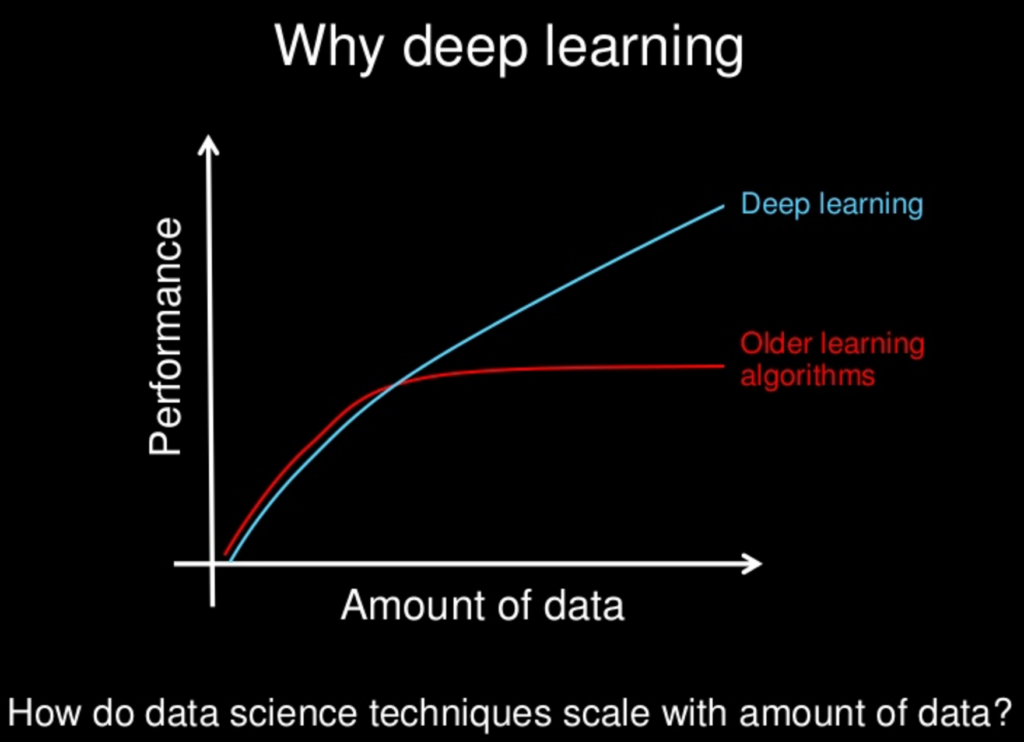
\includegraphics[scale=0.3]{deeplearning_data.png}
	    \caption{Graphe de performance en fonction du nombre de données}
	    \label{fig:data1}
	\end{figure}

    \subsection{Méthodes de complétion}

	Pour ce qui est des différentes méthodes d'augmentation, nous pouvons performer des
	transformations géométriques (translations, symétries, rotations) ou encore des
	déformations pour pouvoir reconnaître les photos prises avec des cameras "fisheyes".
	Il peut être intéressant d'altérer l'intensité de l'image de façon à reconnaître les images
	de test même si elles ont une amplitude d'intensité très variables. Nous pouvons par exemple
	citer la méthode de l'article AlexNet \cite{einstein}


    \subsection{Efficacité de l'augmentation}

	Dans quelle mesure le nombre de données augmentées influent sur la performance ?

\section{Annexes}
%\section{Bibliographie}
%http://ydwen.github.io/papers/WenECCV16.pdf
%https://machinelearningmastery.com/improve-deep-learning-performance/
\bibliographystyle{unsrt}
\bibliography{sample}
%\section{Bibliographie}
%\flushleft [1] http://ydwen.github.io/papers/WenECCV16.pdf 
%\newline
%[2] Zeiler, M. D., \& Fergus, R. (2014, September). Visualizing and understanding convolutional networks. In European conference on computer vision (pp. 818-833). Springer, Cham.
%\newline

\end{document}
